% -*- mode: fundamental -*-

% ****************************************************************

\chapter{RISC-V: the Drum unpipelined CPU}

\markboth{Ch \arabic{chapter}: The Drum CPU code}{\copyrightnotice}

\setcounter{page}{1}
% \renewcommand{\thepage}{\arabic{page}}
\renewcommand{\thepage}{\arabic{chapter}-\arabic{page}}

\label{ch_Drum_code}

% ****************************************************************

\section{Introduction}

So far, we have only been discussing pure combinational functions, for
which there is no concept of time.  Combinational functions are just
pure mathematical functions, ``instantaneously'' transforming input
values to output values.  However, a CPU, as shown in
Figure~\ref{Fig_Drum_Instr_Exec}
\begin{figure}[htbp]
  \centerline{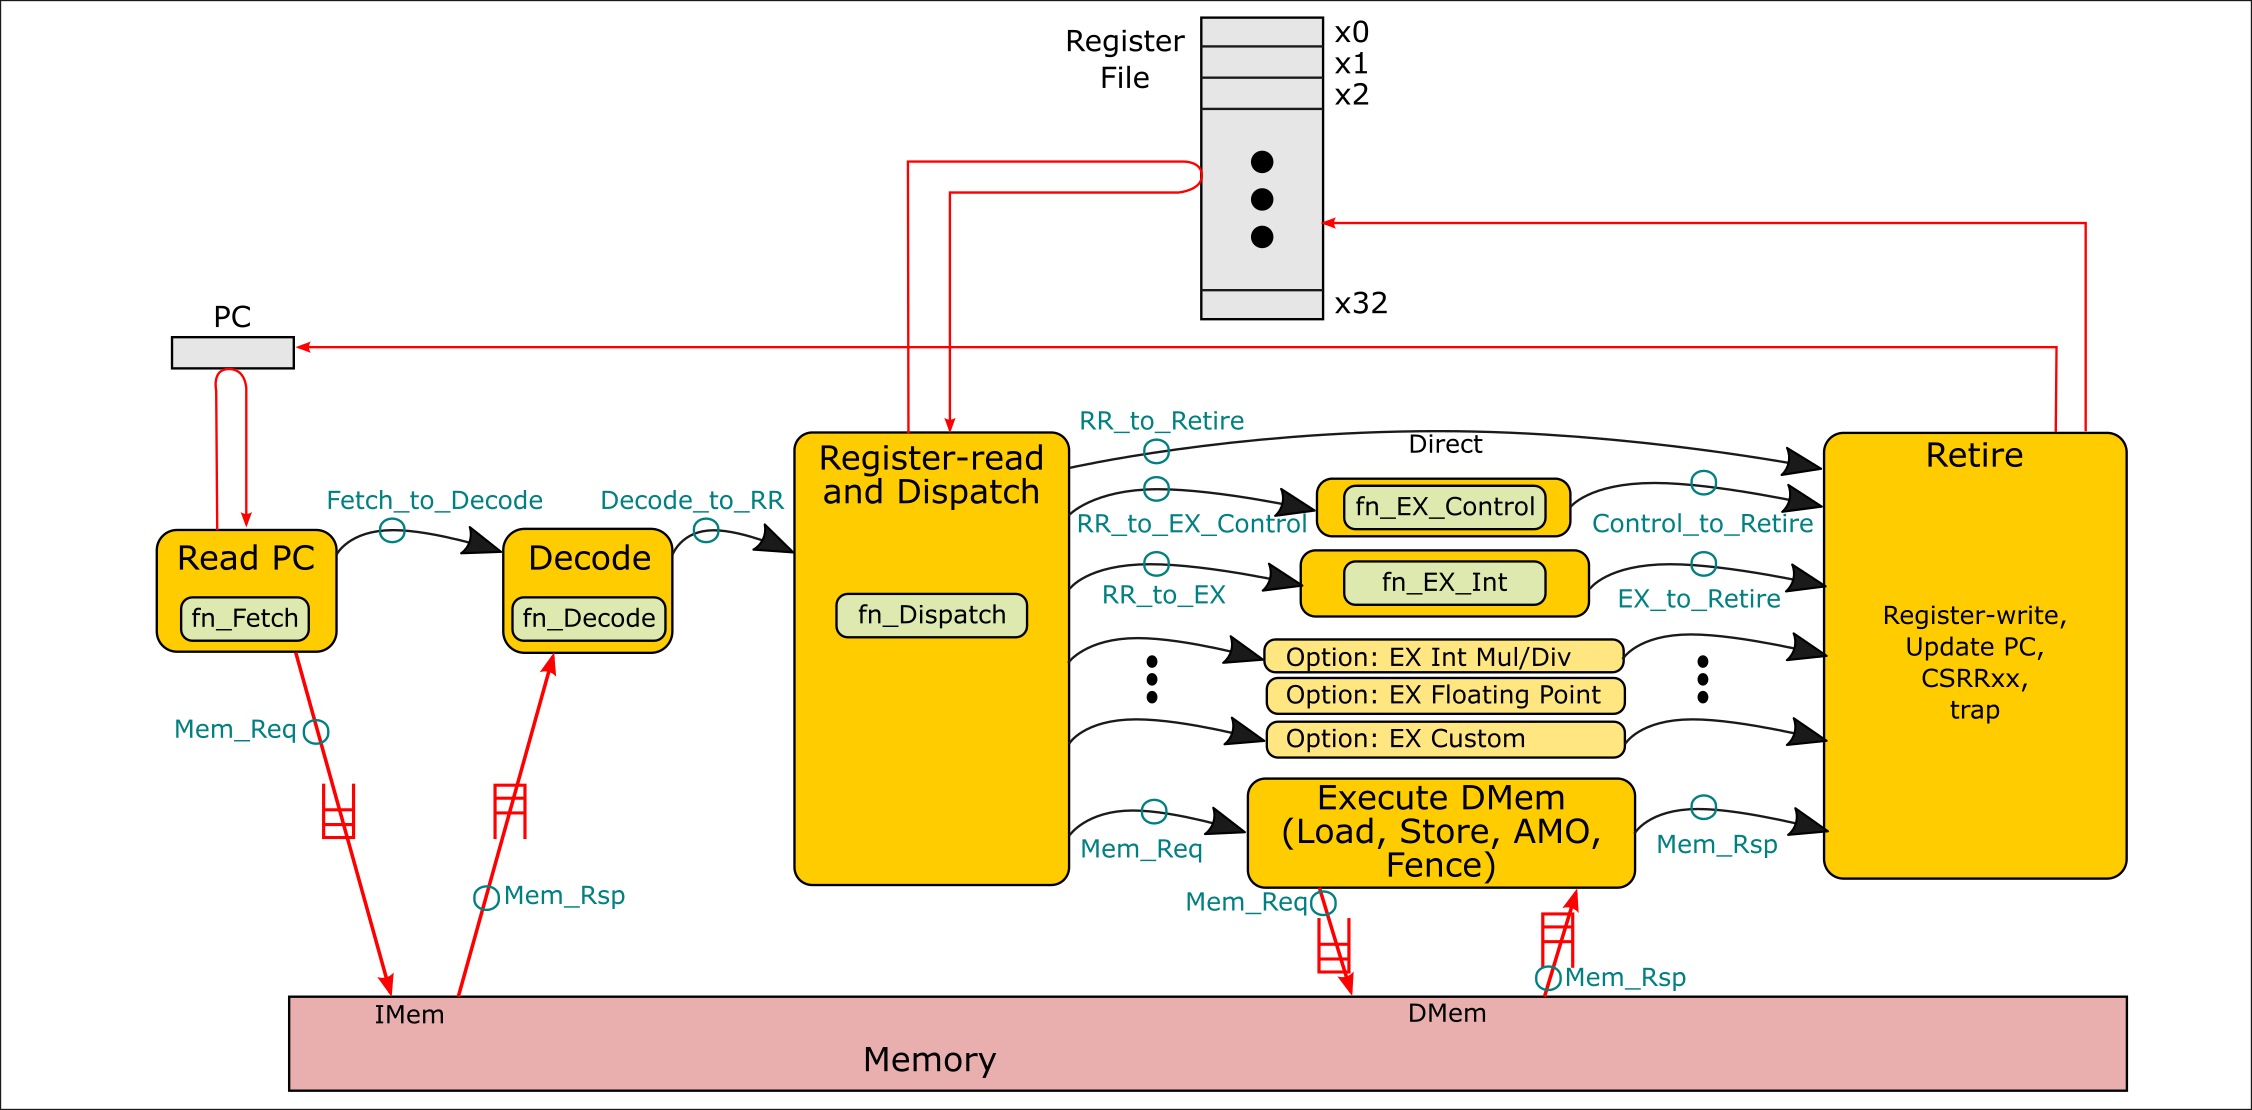
\includegraphics[width=6in,angle=0]{Figures/Fig_Instr_Exec_w_structs}}
  \caption{\label{Fig_Drum_Instr_Exec}
           Simple interpretation of RISC-V instructions
	   (same as Fig.~\ref{Fig_Fetch_function_Simple_Instr_Exec})}
\end{figure}
represents a \emph{processs}, a behavior that evolves over time.  For
example the Drum CPU executes one full instruction after another, and
the black arrows in the diagram represent an infinite loop. For each
instruction, first it performs a Fetch operation, which sends a
request to memory. Some time later, the memory sends back a response,
which is then processed by the Decode step, Register-Read-and-Dispatch
step and then one of the Execute steps.  The Execute Memory Ops step
sends a request to memory. Some time later, the memory sends back a
response, which is processed in the Retire step.  Finally, it it loops
back to the Fetch step, and the process repeats for the next
instruction.

The simplest temporal process in hardware is the FSM (Finite State
Machine).  Figure~\ref{Fig_Drum_Instr_Exec} can be interpreted as an
FSM: each yellow rectangle is a state, and the process transitions
from state to state, thereby executing RISC-V instructions.  This is
exactly what the Drum CPU does.  In this chapter, after first
discussing FSMs in BSV, we discuss the Drum CPU and its FSM
implementation.  By the end of this chapter, we will have a complete
Drum CPU that is capabable of executing RV32I RISC-V programs.

% ****************************************************************

\section{RISC-V: The interface for the Drum and Fife CPU modules}

\label{Sec_Drum_CPU_interface}

Armed with {\tt StmtFSM} we can now complete our description of the
Drum RISC-V CPU, a BSV module.  Before we look at the module, we start
with its interface.  A clean, common interface will allows us later
transparently to substitute the Fife CPU module in place of the Drum
CPU module, and re-use the same test-benches {\etc}

\index{Drum!CPU interface}
\index{Fife!CPU interface}

(Please re-read Section~\ref{Sec_Harvard_architecture} for the
discussion on Harvard architectures, which have separate data channels
for memory-access for instructions (Fetch, IMem) and memory-access for
data (LOAD/STORE, DMem)).

{\small
\begin{Verbatim}[frame=single, numbers=left]
interface CPU_IFC;
   method Action init (Initial_Params initial_params);

   interface FIFOF_O #(Mem_Req) fo_IMem_req;
   interface FIFOF_I #(Mem_Rsp) fi_IMem_rsp;

   interface FIFOF_O #(Mem_Req) fo_DMem_req;
   interface FIFOF_I #(Mem_Rsp) fi_DMem_rsp;
endinterface
\end{Verbatim}
}

The interface is simple:

\begin{tightlist}

  \item The \verb|init| method carries an \verb|Initial_Params| struct
    containing any initial values needed by the CPU.  A typical field
    is the initial value of the PC, since different software systems
    make different assumptions about the ``starting address'' for
    code.  In many RV32I example codes, the starting address is
    \verb|'h_8000_0000|.

  \item A \verb|FIFOF_O| interface to carry memory requests for
    instructions (out-bound from the CPU to the memory);

  \item A \verb|FIFOF_I| interface to carry corresponding memory
    responses containing instructions (in-bound from memory to the
    CPU);

  \item A \verb|FIFO_O| interface to carry memory requests from
    load/store instructions (out-bound from the CPU to the memory);

  \item A \verb|FIFOF_I| interface to carry corresponding load/store
    memory responses (in-bound from memory to the CPU).

\end{tightlist}

% ****************************************************************

\section{RISC-V: The Drum CPU module}

\label{Sec_Drum_CPU_module}

\index{RISC-V!Drum skeleton module}
\index{RISC-V!Fife skeleton module}
\index{Drum!Skeleton module}
\index{Fife!Skeleton module}

Here is the Drum CPU module, except for the BEHAVIOUR section, which
we have elided.  We will fill in the missing piece (a {\tt StmtFSM})
in a following subsection.

{\small
\begin{Verbatim}[frame=single, numbers=left]
(* synthesize *)
module mkCPU (CPU_IFC);
   // ================================================================
   // STATE

   // Don't run until initialized
   Reg #(Bool) rg_running <- mkReg (False);

   // The integer register file
   RISCV_RegFile_IFC  gprs <- mkRISCV_RegFile;

   // The Program Counter
   Reg #(Bit #(XLEN)) rg_pc   <- mkReg (0);

   // Inter-step registers
   Reg #(F_to_D)             rg_F_to_D            <- mkRegU;
   Reg #(D_to_RR)            rg_D_to_RR           <- mkRegU;
   Reg #(RR_to_Retire)       rg_RR_to_Retire      <- mkRegU;

   Reg #(RR_to_Control)      rg_RR_to_Control     <- mkRegU;
   Reg #(Control_to_Retire)  rg_Control_to_Retire <- mkRegU;

   Reg #(RR_to_EX)           rg_RR_to_EX          <- mkRegU;
   Reg #(EX_to_Retire)       rg_EX_to_Retire      <- mkRegU;

   // Paths to and from memory
   FIFOF #(Mem_Req) f_IMem_req  <- mkFIFOF;
   FIFOF #(Mem_Rsp) f_IMem_rsp  <- mkFIFOF;

   FIFOF #(Mem_Req) f_DMem_req  <- mkFIFOF;
   FIFOF #(Mem_Rsp) f_DMem_rsp  <- mkFIFOF;

   // ================================================================
   // BEHAVIOR

   ... // This section will code the dynamic "behavior" of the module
   ... // and will be discussed shortly

   // ================================================================
   // INTERFACE

   method Action init (Initial_Params initial_params);
      rg_pc      <= initial_params.pc_reset_value;
      rg_running <= True;
   endmethod

   interface fo_IMem_req = to_FIFOF_O (f_IMem_req);
   interface fi_IMem_rsp = to_FIFOF_I (f_IMem_rsp);

   interface fo_DMem_NS_req = to_FIFOF_O (f_DMem_req);
   interface fi_DMem_NS_rsp = to_FIFOF_I (f_DMem_rsp);
endmodule

\end{Verbatim}
}

In line 7 we instantiate a register that signals to the BEHAVIOR
section when everything has been initialized and we are ready to start
running.

In line 10 we instantiate the register file using the module
\verb|mkRISCV_RegFile| that was shown in
Section~\ref{Sec_RISCV_regfile}.  In line 13 we instantiates a
register that will serve as our Program Counter.

Lines 12-21 instantiate registers that will hold values between
temporal steps of the FSM.  For example, the Fetch step will write a
value into \verb|rg_F_to_D| which will be read later by the Decode
step.  Not all registers will always contain meaningful values, but
that's OK, each step will read only read from relevant registers at
relevant points in time.

Lines 24-28 contain four FIFOs for IMem requests (outgoing) and
responses (incoming) and DMem requests (outgoing) and responses
(incoming) respectively.  As mentioned before, we do not make any
assumption about the \emph{latency} of memory requests, {\ie} how long
it takes the external memory subsystem to consume a request from one
of the request FIFOs and enqueue a response into the corresponding
response FIFO.

In the INTERFACE section, the \verb|init| method lines 42-45
initializes the PC, and sets \verb|rg_running| to true, releasing the
BEHAVIOR section to start executing.

In lines 39-43 we are using the interface transformers discussed in
Section~\ref{Sec_interface_transfomers} that produce Semi-FIFO
``views'' of FIFOs.

% ================================================================

\subsection{The Drum CPU module behavior}

\label{Sec_Drum_CPU_module_behavior}

\index{RISC-V!Drum CPU module behavior}
\index{Drum!CPU module behavior}

Here we fill in the BEHAVIOR section that was elided in the previous
display.  First we defines a \verb|Stmt| that specifies the execution
of a single instruction (Fetch through Retire):

{\small
\begin{Verbatim}[frame=single, numbers=left]
   Stmt exec_one_instr =
   seq
      // Fetch
      action
	 let y <- fn_F (rg_inum, rg_pc, 0, 0);
	 rg_F_to_D <= y.to_D;
	 f_IMem_req.enq (y.mem_req);
	 rg_inum <= rg_inum + 1;
      endaction
      // Decode
      action
	 let mem_rsp <- pop_o (to_FIFOF_O (f_IMem_rsp));
	 let y       <- fn_D (rg_F_to_D, mem_rsp);
	 rg_D_to_RR <= y;
      endaction
      // Register-Read and Dispatch
      action
	 // Read GPRs
	 // Ok that read_1 and read_2 may return junk values
	 //         since not all instrs have rs1/rs2.
	 let x       = rg_D_to_RR;
	 let rs1_val = gprs.read_1 (instr_rs1 (x.instr));
	 let rs2_val = gprs.read_2 (instr_rs2 (x.instr));

	 Result_Dispatch y <- fn_Dispatch (rg_flog, x, rs1_val, rs2_val);

	 rg_RR_to_Retire  <= y.to_Retire;
	 rg_RR_to_Control <= y.to_Control;
	 rg_RR_to_EX      <= y.to_EX;
      endaction
      // Dispatch to one of the "execute" steps
      if (rg_RR_to_Retire.exec_tag == EXEC_TAG_RETIRE)
	 // No-op
	 action
	 endaction
      else if (rg_RR_to_Retire.exec_tag == EXEC_TAG_CONTROL)
	 // Control
	 action
	    let y <- fn_Control (rg_flog, rg_RR_to_Control);
	    rg_Control_to_Retire <= y;
	 endaction
      else if (rg_RR_to_Retire.exec_tag == EXEC_TAG_IALU)
	 // IALU
	 action
	    let y <- fn_EX_IALU (rg_flog, rg_RR_to_EX);
	    rg_EX_to_Retire <= y;
	 endaction
      else if (rg_RR_to_Retire.exec_tag == EXEC_TAG_DMEM)
	 // DMem
	 seq
	    action
	       Mem_Req y <- fn_DMem_Req (rg_flog, rg_RR_to_EX);
	       f_DMem_req.enq (y);
	    endaction
	    action
	       let mem_rsp <- pop_o (to_FIFOF_O (f_DMem_rsp));
	       let y       <- fn_DMem_Rsp (rg_flog, mem_rsp);
	       rg_EX_to_Retire <= y;
	    endaction
	 endseq
      else
	 action
	    // This should be impossible
	    $finish (1);
	 endaction
      // Retire
      action
	 let y <- fn_Retire (rg_flog,
			     rg_RR_to_Retire,
			     rg_Control_to_Retire,
			     rg_EX_to_Retire);
	 if (y.exception) begin
            // Exception-handling not yet implemented
	    $finish (1);
	 end
	 else begin
	    // Update PC
	    rg_pc   <= y.to_F.next_pc;
	    // Update Rd if has rd-result
	    if (y.to_RW.commit)
	       gprs.write (y.to_RW.rd, y.to_RW.data);
	 end
      endaction
   endseq;
\end{Verbatim}
}

The code is very easy to read, in fact not too different from reading
C/C++ code.  The outer-level corresponds exactly to a left-to-right
reading of Figure~\ref{Fig_Drum_Instr_Exec}:

\begin{tightlist}
  \item an action for Fetch;
  \item an action for Decode;
  \item an action for Register-read-and-dispatch
  \item a nested if-then else performing one of the dispatched flows:
    \begin{tightlist}
      \item a no-op action (in case of direct information from RR to Retire), or
      \item an action for Control; or
      \item an action for IALU; or
      \item a nested \verb|seq| sequence of actions for DMem
        \begin{tightlist}
          \item an action to send a DMem request to memory;
          \item an action to receive a DMem response from memory
        \end{tightlist}
    \end{tightlist}
  \item an action for Retire
\end{tightlist}

Then, we instantiate a \verb|StmtFSM| module that first waits until it
is allowed to run, and then loops forever, executing one instruction
at a time:

{\small
\begin{Verbatim}[frame=single, numbers=left]
import StmtFSM :: *;

(* synthesize *)
module mkCPU (CPU_IFC);

   ...

   // ================================================================
   // BEHAVIOR

   Stmt exec_one_instr = ...;

   mkAutoFSM (seq
                 await (rg_running);
		 while (True) exec_one_instr;
	      endseq);

   // ================================================================

   ...
endmodule
\end{Verbatim}
}

% ----------------
\hdivider

\Exercise

What might happen if we omitted the ``{\tt await!(rg\_running)}''
statement in the Drum CPU? (Try it in simulation!)

\emph{Hint:} The FSM may start running before the PC has been initialized ...

\Endexercise
% ----------------

Retire actions in Drum

\begin{figure}[htbp]
  \centerline{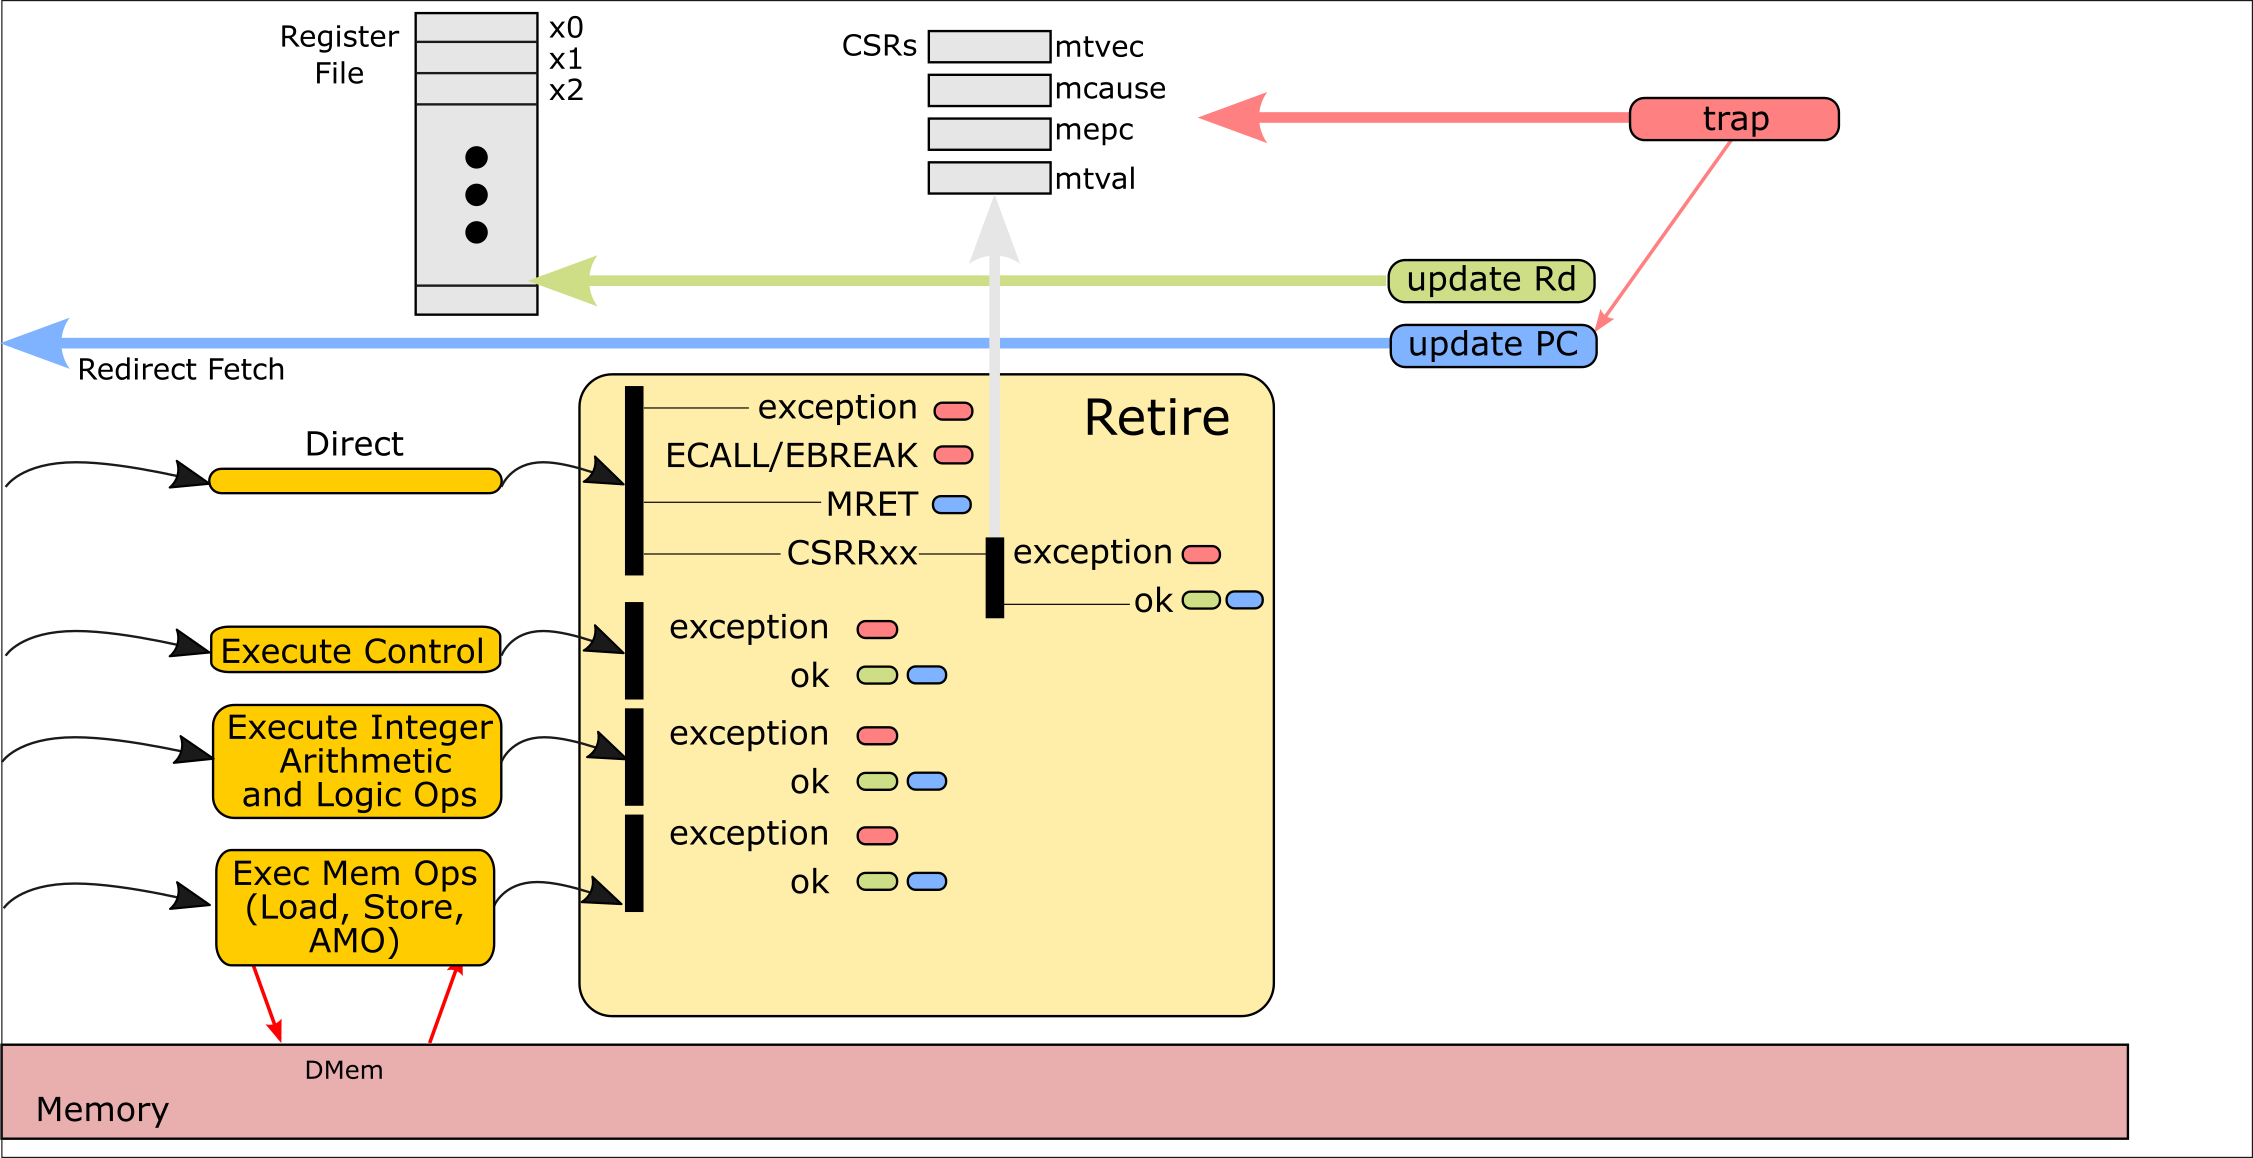
\includegraphics[width=6in,angle=0]{Figures/Fig_Retire_Layers_1}}
  \caption{\label{Fig_Retire_Drum}Retire actions in Drum}
\end{figure}

% ****************************************************************

\section{RISC-V: Comparing Drum BSV CPU to C code for a RISC-V simulator}

... TO BE WRITTEN ...

% ****************************************************************
